\chapter{The CMS experiment at the \LHC}
\label{chap:detector}

% \chapterquote{There, sir! that is the perfection of vessels!}
% {Jules Verne, 1828--1905}

To be able to reliably probe the energy scales at which the \SM breaks
down, one of the largest machines ever built was constructed in a
27~km ring underground on the border of France and Switzerland: the
\LHC. Along this are built a series of detectors that can record in a high
level of detail the result of high energy particle collisions produced
by this collider. This chapter will focus on the details and
performance of \CMS, a multi-purpose detector optimised to search for
new, as yet undiscovered, particles.

\section{The \LHC}
\label{sec:lhc}

The \LHC is a hadron collider designed to collide protons and lead
ions at energies up to 14\tev, the highest ever achieved by such a
machine
\cite{Evans:2008zzb,CERN-2004-003-V-1,CERN-2004-003-V-2,CERN-2004-003-V-3}.
The proton-proton collisions are most utilised for direct searches for
new physics and therefore take up the vast majority of the \LHC's
running time. 

To bring protons up to the $6.5\tev$ required per beam in Run~2 of
the \LHC they are accelerated through a series of steps. Protons are
initially taken from a bottle of hydrogen, ionised and accelerated to
50\mev by a linear accelerator, \ac{LINAC2}. The energy is then boosted to
1.4\gev by the \ac{PSB} before being injected into the \ac{PS} which
brings the energies up to 26\gev. A final kick up to 450\gev is
provided by the \ac{SPS}. The protons are then injected into the \LHC
in bunches, prepared by the previous accelerators, that are either
25~ns (from Run~2 onwards) or 50~ns apart (during Run~1 and early
stages of Run~2). The protons are steered within the \LHC ring by
around 1200 superconducting dipole magnets while being accelerated up
to $6.5\tev$ with \ac{RF} cavities. Protons are bought to collide at
four different points on the ring, around which are built the four
major \LHC experiments, ALICE \cite{Aamodt:2008zz}, ATLAS
\cite{Aad:2008zzm}, LHCb \cite{Alves:2008zz} and \CMS
\cite{Chatrchyan:2008aa}.

\begin{figure}
  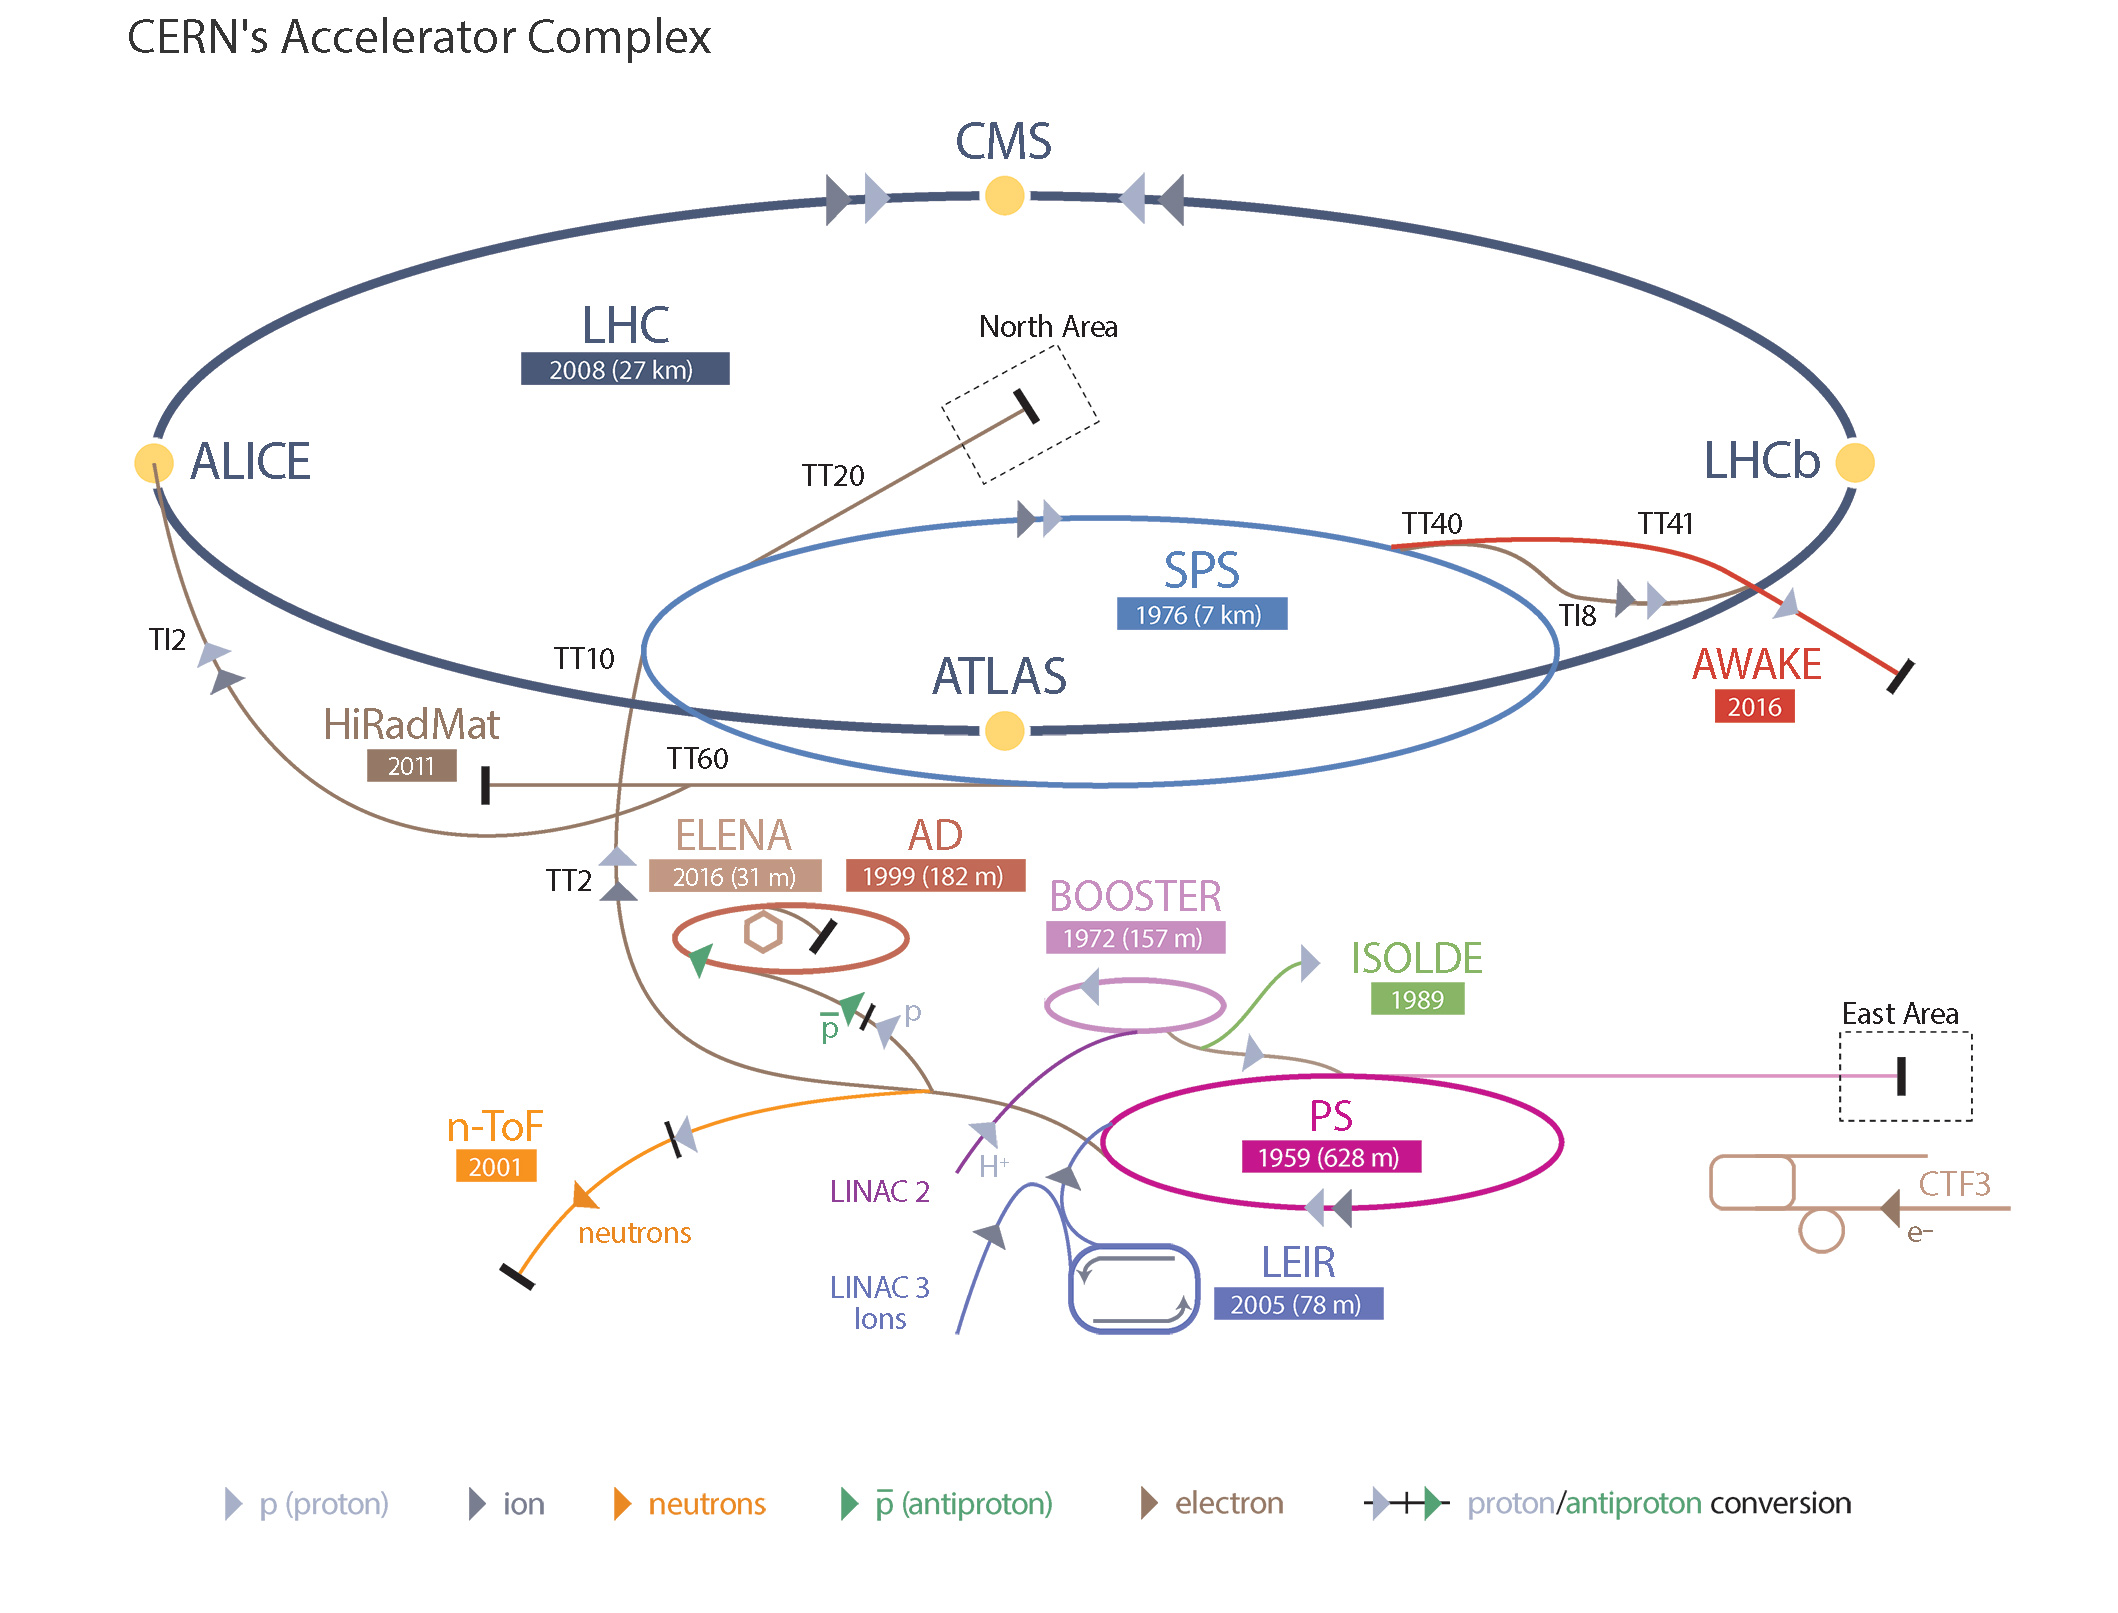
\includegraphics[width=\largefigwidth]{figs/LHC_default}
  \caption[]%
  {A representation of the CERN accelerator complex that help
  accelerate protons to record energies within the \LHC
  \cite{stfc:lhc}}%
  \label{fig:lhc}
\end{figure}

Another key design feature of the \LHC is the very high rate at which
hadrons are collided. lumi stuff... trigger

Datasets in this analysis...

\cite{Evans:2008zzb} 

% \begin{figure}
%   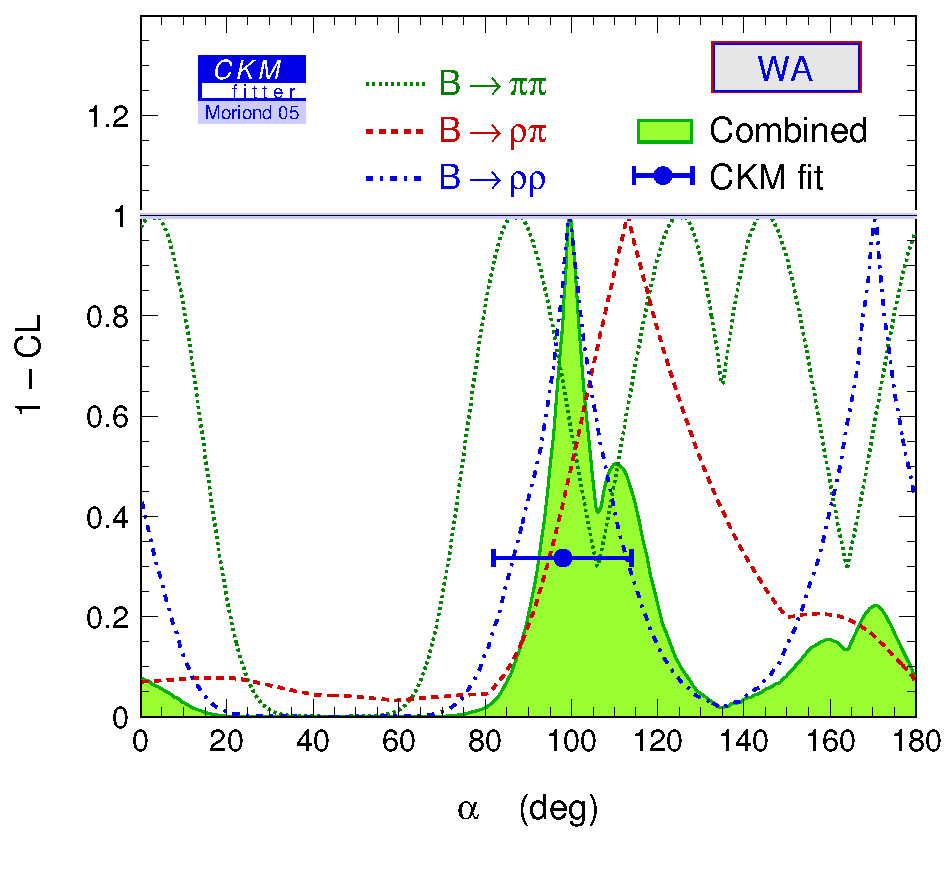
\includegraphics[width=\largefigwidth]{ckmfitter-alpha-combined}
%   \caption[CKM Fitter constraints on \alphaCKM.]%
%   {CKM Fitter constraints on \alphaCKM from combined \BToPiPi,
%     \BToRhoPi and \BToRhoRho decay analyses.}
%   \label{fig:CKMFitter}
% \end{figure}

\section{The CMS detector}
\label{sec:cms}

\subsection{Trigger system}
\label{sec:triggers}

% \begin{table}[bp]
%   \begin{tabular}{lllll}
%                 & L0              & L1              & HLT             \\
%     \midrule\\
%     Input rate  & \unit{40}{\MHz} & \unit{1}{\MHz}  & \unit{40}{\kHz} \\
%     Output rate & \unit{1}{\MHz}  & \unit{40}{\kHz} & \unit{2}{\kHz}  \\
%     Location    & On detector     & Counting room   & Counting room   \\
%   \end{tabular}
%   \caption{Characteristics of the trigger levels and offline analysis.}
%   \label{tab:TriggerDetails}
% \end{table}
